\documentclass[a4paper,12pt]{extarticle}

\usepackage[T1]{fontenc}
\usepackage[utf8]{inputenc}

\usepackage[]{parskip}
\usepackage{hyperref, wrapfig, float, amsmath, adjustbox, array, pdflscape, soul, color, extsizes}
\usepackage{booktabs}
\usepackage{multirow}

\renewcommand{\arraystretch}{2}
\renewcommand{\contentsname}{Spis treści}
\renewcommand{\refname}{Bibliografia}
\renewcommand{\figurename}{Rys.}
\renewcommand{\tablename}{Tab.}

\usepackage{geometry}
\geometry{
  a4paper,
  margin=20mm,
  bottom=30mm
}

\usepackage{graphicx}
\usepackage{caption}
\usepackage{subcaption}
\usepackage[font=small,labelfont=bf]{caption}
\graphicspath{ {./images/}{../images/} }

\newcommand{\mathcolorbox}[1]{
  \begin{center}
    \colorbox{yellow}{$\displaystyle #1$}
  \end{center}
}
\newcommand{\pvec}[1]{
  \vec{#1}\mkern2mu\vphantom{#1}
}
\newcommand{\angstrom}{\mbox{\normalfont\AA}}

\begin{document}
  \begin{titlepage}
    \begin{center}
      \begin{figure}[H]
        \centering
        
\includegraphics[scale=.125]{logopp.png}
      \end{figure}
      \vspace*{.05\textheight}
      \huge\textbf{Politechnika Poznańska}\\
      \large\textbf{Wydział Inżynierii Materiałowej i Fizyki Technicznej}\\
      \large\textbf{Fizyka Techniczna}\\
      \vspace*{.2\textheight}
      \huge\textbf{Modelowanie cząsteczki \( C_6H_{12} \)}\\
      \vspace*{.025\textheight}
      \large\textbf{Jakub Bąbelek\\(nr.\ albumu: 136454)}
    \end{center}
  \end{titlepage}
  
  \clearpage
  \section{Wstęp}
  Cykloheksan to organiczny związek chemiczny, jest on nasyconym węglowodorem
  alicyklicznym zawierającym 6 atomów węgla oraz 12 atomów wodoru. Atomy węgla
  znajdują się w hybrydyzacji \( sp^3 \) i każdy z nich posiada po 4 wiązania.
  Aby cząsteczka była stabilna musi znajdować się ona w jednej z konformacji (ułożenia geometrycznego)
  jak np. krzesło, łódka czy skręcona łódka. Nazwy te pochodzą od wyglądu cząsteczki po
  wykonanych obliczeniach. Różne formy geometryczne cykloheksanu zostały zaobserwowane
  po raz pierwszy przez Sachsa w 1890 roku.

  \noindent Do modelowania molekuły \( C_6H_{12} \) użyliśmy 2 metod:
  \begin{enumerate}
    \item
    AM1 (Austin Model  1) - Półempiryczna metoda kwantowa służąca do obliczeń struktury elektronwej.
    Głównym jej założeniem jest formalizm Hartee-Focka.
    
    \item
    PM3 (Parametric Model 3) - Półempiryczna metoda kwantowa służąca do obliczeń struktury elektronwej.
    Metoda podobna do AM1 lecz używająca innych wartości parametrów formalizmu Hartee-Focka.
  \end{enumerate}

  \section{Wyniki}

  Poniższa tabela porównuje energię całkowitą oraz ciepło tworzenia dla obu użytych
  metod i wszystkich badanych konformacji.

  \begin{table}[H]
    \centering
    \begin{tabular}{cccccc}
    \toprule
    \multicolumn{2}{c}{\textbf{Metoda}}                                                                               & \textbf{Krzesło} & \textbf{Łódka} & \textbf{Skr. łódka} & \textbf{Płaska} \\
    \midrule
    \multirow{2}{*}{\begin{tabular}[c]{@{}c@{}}Energia\\ Całkowita \([\frac{kcal}{mol}]\)\end{tabular}}       & AM1 & -21556.7926      & -21553.1789    & -21553.5304         & -21541.3402     \\
                                                                                                                & PM3 & -20688.4638      & -20684.0239    & -20684.3753         & -20671.368      \\
    \midrule
    \multirow{2}{*}{\begin{tabular}[c]{@{}c@{}}Energia\\ Termodynamiczna \([\frac{kcal}{mol}]\)\end{tabular}} & AM1 & -36.4943         & -32.8806       & -33.2321            & -21.0418        \\
                                                                                                                & PM3 & -30.4391         & -25.9992       & -26.3506            & -13.3433        \\
    \bottomrule
    \end{tabular}
  \end{table}

  \begin{figure}[H]
    \centering
    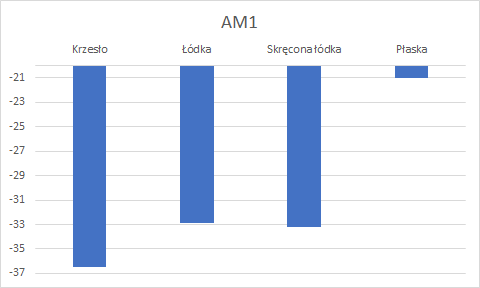
\includegraphics[width=10cm]{am1.png}
    \caption{Ciepło tworzenia dla metody AM1 \([\frac{kcal}{mol}]\)}
    \label{fig:am1}
  \end{figure}

  \begin{figure}[H]
    \centering
    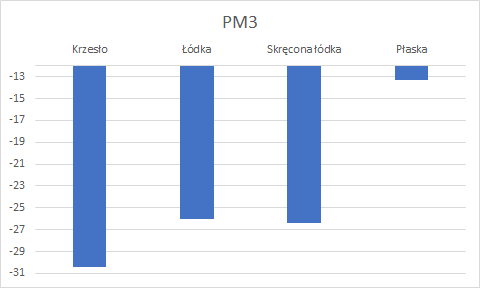
\includegraphics[width=10cm]{pm3.png}
    \caption{Ciepło tworzenia dla metody PM3 \([\frac{kcal}{mol}]\)}
    \label{fig:pm3}
  \end{figure}

  Widzimy, że oba wykresy są właściwie indentyczne. Różnice liczbowe wynikają z
  dokładności użytych metod.

  \begin{figure}[H]
    \centering
    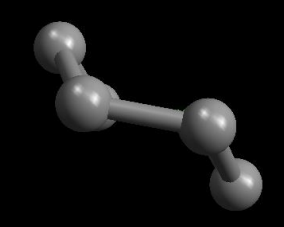
\includegraphics[width=5cm]{krzeslo.png}
    \caption{Konformacja --- krzesło (ukryte wodory)}
    \label{fig:krzeslo}
  \end{figure}

  Poniższe konformacje do uzyskania potrzebowały zmiany geometrii cząsteczki przez
  np. przemieszczanie lub obracanie grup wodorowych (konformacja pierwsza
  (\figurename\ref{fig:krzeslo}) posiada najmniejszą energię przez co symulacja
  najłatwiej uzyskuje właśnie taki wynik)

  \begin{figure}[H]
    \centering
    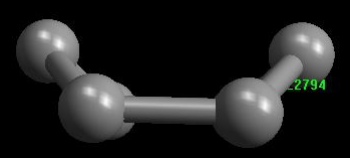
\includegraphics[width=5cm]{lodka.png}
    \caption{Konformacja --- łódka (ukryte wodory)}
    \label{fig:lodka}
  \end{figure}

  \begin{figure}[H]
    \centering
    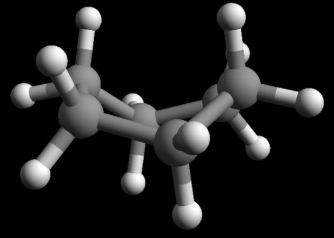
\includegraphics[width=5cm]{skr_lodka.png}
    \caption{Konformacja --- skręcona łódka}
    \label{fig:skr_lodka}
  \end{figure}

  \begin{figure}[H]
    \centering
    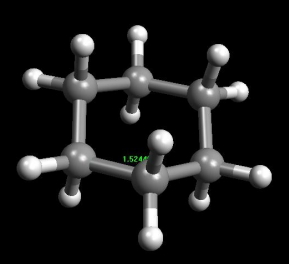
\includegraphics[width=5cm]{plaska.png}
    \caption{Konformacja --- płaska/planarna}
    \label{fig:plaska}
  \end{figure}

  \section{Wnioski}
  Przeprowadzone symulacje pokazały, że niektóre metody w tym przypadku są znacznie
  lepsze. Optymalizacja UFF nie dawała poprawnych wyników. Jedynie metody kwantowe
  AM1 oraz PM3 pozwoliły na uzyskanie poprawnych danych. Wyniki dla obu metod są
  zbliżone i różnią się bardzo niewiele. Znalezione konformacje wymagały ręcznej modyfikacji
  geometrii cząsteczki (szczególnie problematyczna okazała się konformacja łódki)
  tak aby można było uzyskać konformacje inne niż krzesło (najłatwiejsza konformacja
  do uzyskania z naniższą energią całkowitą)

  \begin{thebibliography}{9}
    \addcontentsline{toc}{section}{Bibliografia}
        
    \bibitem{arguslab}
    Obliczenia i wizualizacje zostały wykonane za pomocą:\\
    \textit{ArgusLab 4.0}\\
    Mark A. Thompson\\
    Planaria Software LLC, Seattle, WA.
    http://www.arguslab.com
  \end{thebibliography}

\end{document}